
% Many thanks to Andrew West for writing most of this file
% Main LaTeX file for CIS400/401 Project Proposal Specification
%
% Once built and in PDF form this document outlines the format of a
% project proposal. However, in raw (.tex) form, we also try to
% comment on some basic LaTeX technique. This is not intended to be a
% LaTeX tutorial, instead just (1) a use-case thereof, and (2) a
% template for your own writing.

% Ordinarily we'd begin by specifying some broad document properties
% like font-size, page-size, margins, etc. -- We have done this (and
% much more) for you by creating a 'style file', which the
% 'documentclass' command references.
\documentclass{sig-alternate}
 
% These 'usepackage' commands are a way of importing additional LaTeX
% styles and formattings that aren't part of the 'standard library'
\usepackage{mdwlist}
\usepackage{url}
\usepackage{float}
\usepackage{listings}

\begin{document} 

% We setup the parameters to our title header before 'making' it. Note
% that your proposals should have actual titles, not the generic one
% we have here.
\title{Programming Language Support for Probabilistic Associative Memory}
\subtitle{Dept. of CIS - Senior Design 2014-2015\thanks{Advisor: Steve A. Zdancewic (stevez@cis.upenn.edu).}}
%\thanks{ Do not list your advisors amongst the authors as that may cause Google Scholar to add this work to their list of publications. Your advisor must also sign a hard-copy of your proposal.}}
%\thanks{ }}
\numberofauthors{3}
\author{
    Fan Yin \\ \email{fanyin@seas.upenn.edu} \\Univ. of Pennsylvania \\ Philadelphia, PA
    \and Haolin Lu \\ \email{haolinlu@seas.upenn.edu} \\Univ. of Pennsylvania \\ Philadelphia, PA
    \and Yukuan Zhang\\ \email{yukuan@seas.upenn.edu} \\Univ. of Pennsylvania \\ Philadelphia, PA
}
%\author{
%\alignauthor Radoslav Ivanov \\ \email{rivanov@seas.upenn.edu} \\ Univ. of Pennsylvania \\ Philadelphia, PA 
%
%\and Radoslav Ivanov \\ \email{rivanov@seas.upenn.edu} \\ Univ. of Pennsylvania \\ Philadelphia, PA 
%
%}
\date{}
\maketitle

% Next we write out our abstract -- generally a two paragraph maximum,
% executive summary of the motivation and contributions of the work.
\begin{abstract}
    The goal of this project is to create a programming language library that provides an interface
    for programming with a probabilistic associative memory, as well as various implementations of these memories. 
    An associative memory allows queries by content rather than by address or location.
    Probabilistic associative memory returns a value based on a probability model
    for a given memory query. This project provides an intuitive interface to this probabilistic
    associative memory to facilliate programming efficiency for the end user.

\end{abstract}

\section{Introduction}
\label{sec:intro}

The standard way to access a stored value in memory is by address. 
This involves finding the physical position of that address in memory
and returning the stored value. Meanwhile, associative memory allows
searching for values based on the stored content. An analogous structure
in programming languages is the hashtable, which returns an output value
based on an input key. 

Standard associative memories are useful for when one needs to query memory based 
on some input data or tag. For instance, router firmware often employs associative 
memories to store tables of Internet Protocol (IP) addresses, which serve as the ``next hop" for incoming 
packets. Since routers looking for the ``next hop" have a specific, standard query 
format -- e.g. an IP address of the form www.xxx.yyy.zzz -- it makes sense to store the 
routing tables based around this input string.

A probabilistic associative memory differs from an associative memory in the sense that 
values stored in the latter are not guaranteed to be recalled with 100-percent fidelity.

For instance, suppose there existed some database of words where ``kat" appeared once and the word ``cat" appeared 100 times.
If this collection were stored within a regular associative memory, and the memory is queried for a string matching ``kat", the memory 
would return ``kat" because it was stored in the memory. With a probabilistic memory, the same query may return ``cat", simply because 
''cat" matches closely with ``kat" and it occurs much more often. The word ``cat" would thus be considered the more ``likely" match.
Thus, with probabilistic memories, the most ``likely" value is returned for a given query based on some probability model of the values
stored in memory.

%Since our queries work directly with a probability model, it would offer more fluidity
%with programming that involves statistical modeling or simulations. 
%Returning values based on a probability also saves memory because not every value has to be stored. 
In a simplistic representation of a probability model, a frequency table of memory values can be constructed as memory values are stored.
The queries would then consist of a set of values, and a likelihood would be generated based on both frequency and some matching metric in that query-set.
Thus, the memory mechanism can extrapolate or interpolate a response to a query based on values 
previously inserted into memory. 

%See Figure 1 for a representation of the flow of this probabilistic mechanism.

The implementation may also include support for structured data in the probabilistic associative memory.
In a standard associative memory scheme, a similarity query is done by comparing input bits
to the values stored in memory. However, this does not allow for accurate similarity comparisons
between trees or lists, as the memory is not aware of the underlying structure. As a result,
many applications on structured data will first flatten the structure, perform the requisite 
calculations, then reconstruct the original structure of that data. With a built-in type system
that supports structured data, the user will be able to directly manipulate the data in memory 
while keeping the structure intact.

Practical applications of probabilistic associative memories involve various approximation and prediction methods.
These involve appliactions such as image reconstruction from noisy input data, or search autocompletion.
This project strives to provide a simple, flexible interface to work with these probabilistic associative memories.



\section{Related Work}
\label{sec:related_work}

With regards to existing related work, the goal of this project is not to advance associative memory techniques.
Rather, it is seeking to research existing models for associative memory, provide a simple probabilistic query interface, and create 
implementations that fit this interface. With that in mind, there are many works that address different forms of associative memory. 

\subsection{Founding Research}
\label{subsec:founding}

One of the seminal works concerning associative memories is Willshaw's \textit{Non-holographic
Associative Memory}~\cite{holographic}. This paper describes a model for a probabilistic associative memory
that holds relations between elements of a query space and elements of an output space. A query
to the memory comes in the form of an element in the query space, and the memory returns the
output that was most likely related to the query element, with a certain degree of confidence.
This model also guaranteed that if a query element was never stored in the memory, a relation
would not be found for that element, with the same degree of confidence as above.

Willshaw's paper was the first to present a model for emulating an associative memory
probabilistically, without storing each element pair explicitly,
and much of the following research on memory compression methods
for probabilistic associative memory were based on this work. While Willshaw's model
enforced a strict mapping between the stored elements, later work also found ways to
give likely matches for elements which the memory has never seen.

\subsection{Modern Connections}
\label{subsec:modern}

Research in associative memory has close connections to neural networks. Our brains function as 
associative memories that can retrieve memories based on similarity between stimuli and the memories themselves. 
Indeed, Norman and Bobrow~\cite{bobrow} construct a memory model which describes how minds retrieve 
items in memory from partial descriptions, even if some part of the description is incorrect or inaccurate. 

Applying this memory model to computation, Hinton~\cite{hinton} draws a connection between Norman and Bobrow's idea of 
retrieving memories based on partial descriptions and content-addressable memories.
Hinton then notes that although this content-addressable memory is a useful representation,  
it is difficult to efficiently ``search for content" through a memory space. 
%In this model, memory is a ``pattern of activity" that constructs the most plausible process based on the given memory queries. 
Hinton ends by claiming that while this model is conceptually not difficult, it is difficult to actually 
implement it. He mentions that an approach to this problem that has arisen recently is with stochastic processes 
-- heralding a probabilistic approach to this associative memory problem. Thus, both Willshaw and Hinton offer probabilistic models
of dealing with associative memories.

\subsection{Implementations}
\label{subsec:implementations}
Later on, the development of Hopfield networks introduced a new form of neural network
that handles associative memory. These neural networks may be used as content-addressable memory by
storing memories on a constant number of nodes and connections, with a similar loss of 
fidelity as the Willshaw paper's model. While it had been shown that the theoretical maximum capacity for these networks
can asymptotically approach twice the network size~\cite{gardner}, the initial Hopfield model 
provided relatively low capacity. Work by Palm~\cite{palm} details the history of 
neural associative memories (including the Willshaw model), the limitations of the initial Hopfield model, and the improvements
that have been made upon it. Namely, it mentions using the Hebb learning rule over the original
Hopfield learning rule and the importance of sparse coding of patterns. 

Sparse coding in particular is quite important in Hopfield networks (and in unsupervised
machine learning in general). For various applications, it is beneficial to utilize
structural similarities to represent the input in a smaller space. In particular, quite 
accurate reconstructions can be created from damaged or noisy images, where details that were 
not even present in the input can be recovered. While this particular example primarily has its uses in, say, 
medical imaging~\cite{yang}, sparse coding has been incredibly useful in increasing the
capacity of these neural associative memories. 


\section{Project Proposal}
\label{sec:project_proposal}
The OCaml language will be used to implement this probabilistic associative memory. 
Based on the specific probability distribution and model in use, the library would return 
a different memory value for each query.
As such, our library will have user-defined support for different probability paradigms. 
After the library is created, applications will be created with the library to demonstrate the benefits of using this implementation
of probabilistic associative memory.

\subsection{Anticipated Approach}
\label{subsec:approach}

The first step is to create a programming language interface for probabilistic
associative memories. This involves implementing a domain specific language: 
defining a type system as well as a syntax for programming with an underlying memory.
A major component of this syntax will be the grammar of memory storage, 
as well as the different types of queries that can be made to the memory. The complexity allowed
within our query interface is of particular importance, as it directly
interfaces with the probability model. Thus, we must carefully consider 
how additional complexity may be implemented within models. 

On a basic level, there are certain required operations that need to be 
supported, such as creation of a memory and storage of values. Moreover,
there must be some form of querying, with at least basic support for querying
for a literal equality match. A diagram of the interface can be shown in Figure 1.

Additional complexity can be added with support for OCaml's pairs and the 
ability to query for a match of the left, right, or both parts of the pair. Functions that transform
queries using logical operations may be added as well. 

\begin{figure}[H]
	\begin{center}
		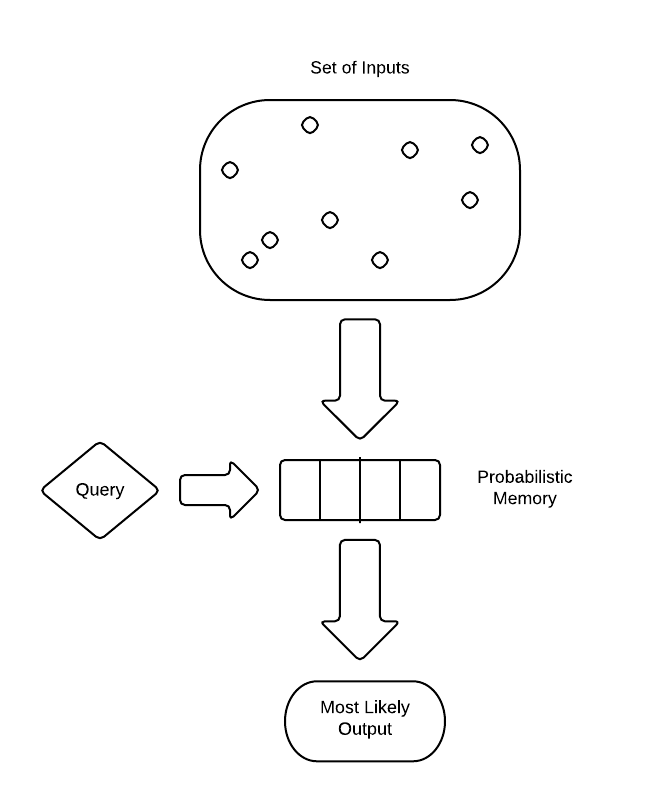
\includegraphics[width=1\linewidth]{pammodel}
	\end{center}
	\vspace{-12pt}
	\caption{Model of Probabilistic Associative Memory Mechanism}
	\label{fig:pammodel}
\end{figure}

Perhaps a very significant source of complexity would come from advanced
queries, which raises the question
of how they may be implemented. 
As a simple example, queries for matching strings can be implemented in varying 
degrees of complexity - from simple literal matching, to wildcard matching, to
entire regex evaluation. For generic datatypes as supported in this presented
library, the issue becomes much more difficult. We anticipate requiring user
input in order to determine how to calculate similarity, much like how 
supervised machine learning algorithms require features to be decided. 
While this does
introduce an extra requirement for use, it will allow easy integration with
structured data such as lists or trees. Alternatively, a form of feature
selection may be useful, although usefulness may be limited without knowledge
of the data type. 

After the design stage, we will implement various types of probabilistic associative memories.
An initial example implementation of the interface may be a deterministic version that
ensures fidelity and keep track of every value that
was stored in it. Later implementations will try to conserve memory space,
and compress the stored values. We will work on several different data representation methods,
including those related to neural networks. 

By creating this interface, users of this programming language will be able to
choose the type of memory and probabilistic model that most suits the needs of their particular
application. Moreover, it will allow users to implement the interface with their own models as necessary, 
as well as provide easy usage of the provided probabilistic models (Figure 2).

\begin{figure}[H]
	\begin{center}
		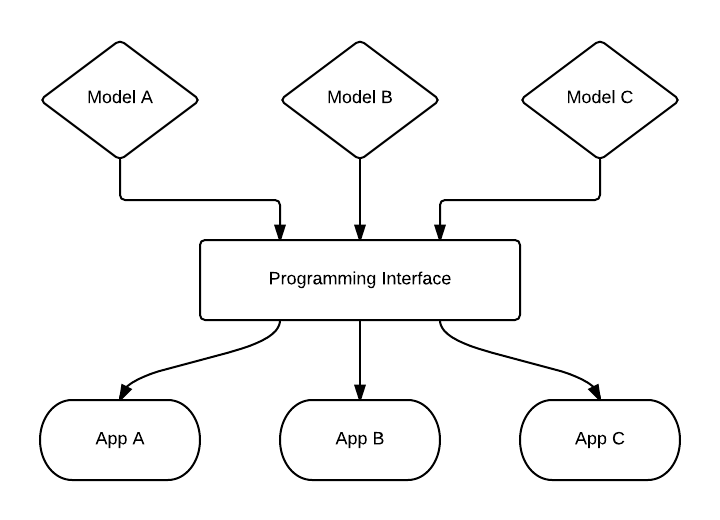
\includegraphics[width=1\linewidth]{block2}
	\end{center}
	\vspace{-12pt}
	\caption{Programming Pipeline of our Library}
	\label{fig:block2}
\end{figure}

\subsection{Technical Challenges}
\label{subsec:tech_challenges}
The foremost technical challenges in our project involve creating the programming interface,
the logistics of incorporating probabilistic models into the memory mechanism, and
the mathematics involved in these models.

Regarding the interface that the end user (programmer) sees, she should not have to be aware of 
the inner workings of each probabilistic model, but expect reasonable and intuitive return values
to each query into the probabilistic memory. For instance, if she is prioritizing accuracy 
in her use of the library, she would expect a return value that was previously inserted and that 
returns the highest probability for the given query.

However, it is also necessary to give the programmer enough power and flexibility with our library for 
whatever probabilistic applications she will be using it for. This involves enabling 
her to create query combinations and queries of different types. Still, flexibility may 
come at the cost of complexity - implementing features to accommodate arbitrary data, queries,
and probabilistic models quickly increases the complexity of this project. 

Regarding mathematics, it is necessary to further research mathematical 
and probabilistic methods that would be implemented in this library. After implementing these methods,
we will need to verify that mathematical or probabilistic models behave as expected. 
For instance, if the previous values inserted into a high-fidelity probabilistic memory were ``2, 2, 2, 4, 4, 6", and we queried ``x > 2", 
then the return value based on a specific probabilistic model should be ``4", since ``4" is the most frequent value that satisfies the query.
Of course, in our actual implementation, we will have more complicated mechanisms than the one above.
Thus, another challenge involves testing, through confusion matrices or other machine-learning techniques,
that our return values achieve a certain standard of accuracy or fidelity.

\subsection{Evaluation Criteria}
\label{subsec:eval_criteria}
There are two main criteria which, combined, makes this library novel and effective. 
The first criterion is that it provides comparable results to other associative memory techniques. 
For instance, an autocomplete program (of sentences) can be written with this library and compared against an existing implementation of autocompletion. 
Evaluating the correctness and results of these autocompletion programs may involve taking a collection of existing sentences and truncating them
at certain places. First, a set of training data along with the truncated sentences will be passed into both autocompletion programs. 
Then, the percentage of words that each program autocompleted correctly will be returned as the evaluation metric. 

The second criterion, which is the main focus of the library, involves simplifying the programming interface for associative memory techniques.
To evaluate this criterion, we will analyze how generic our code is. That is, given an autocompletion program, suppose one wanted to adapt this 
program for recognizing a melody based only on a musical fragment or phrase. Ideally, the library would facillitate minimal changes to the existing 
autocompletion program. The user would only need to provide different functions for evaluating the data, and the rest of the framework can remain as it is. 

The utility of this library lies in its generality in implementing associative memory techniques. While this project does not attempt to improve 
existing associative memory algorithms, it seeks to provide a simple, flexible interface for implementing associative memory applications.

%We do not plan on improving on the capabilities of modern associative memory
%systems, but these benchmarks should show that we approach implementations of similar
%quality. 

%Regarding other metrics, it will be shown how this probabilistic library can yield 
%fewer lines of code and has more logical fluidity for programs that require statistical
%and probabilistic methods than a vanilla implementation of the same program in OCaml. 

%Regarding benchmarks, we will attempt to show how the probabilistic approach may lead to 
%a lower memory footprint, but still return values similar to an expected baseline.

%For instance, we might begin by programming a simple dice-rolling application where the programmer wishes
%to simulate an unfair six-sided dice, i.e. where the probability of rolling a number from 1 to 6 is not $\frac{1}{6}$.
%The function of this application is twofold: by running the simulation through multiple trials, it can be demonstrated 
%that this probability model works correctly; that is, that it generates the expected distribution values
%based on the given inputs. In addition, the logical fluidity of using the probabilistic library will be demonstrated:
%With a standard programming model, this loaded dice simulation might require many lines of casework and probability space scaling
%that ends up being unintuitive. For example, say we wanted to assign ''1" to show up with probability $\frac{1}{3}$
%and the other numbers with probability $\frac{2}{15}$. With a standard programming model, we would have to run the simulation on a space from
%1 to 15, instead of 1 to 6, and essentially map $\{1\} \rightarrow \{1, 2, 3, 4, 5\}, \{2\} \rightarrow \{6, 7\}$, etc...

%With this library, the programmer would be able to accomplish this much more intuitively. Listing 1 shows a potential representation of how we might use the library interface. Our
%anticipated user interface would provide an abstraction such that the programmer would simply
%provide the probability distribution that she desires.

%\lstset{language=Caml, caption={Code for Dice Example}, captionpos=b, xleftmargin=\parindent, xrightmargin=\parindent}
%\begin{lstlisting}[frame=single]
%let create (distribution : [Int]) =
%    let mem = new[Int] in
%        storeList(mem, distribution);
%        mem
%let loadedDie = create [1,1,2,3,4,5,6]
%query(loadedDie) ==> (* 1 is twice as 
%    likely to appear as the other 
%    numbers *)
%\end{lstlisting}

\section{Research Timeline}
\label{sec:research_timeline}
%Finally, we would like you to speculate about the pace of your
%research progress. This section need not be lengthy, we would just
%like you to specify some milestones so we can gauge your progress
%during our intermediate interviews. Let us follow through with our
%image recognition example:

% The 'itemize' environment shown here, and its friend 'enumerate'
% (shown below), are used to create indented\bulleted\outline style
% lists.
\begin{itemize*}
	\item {\sc already completed}: Preliminary reading and research. Brainstorm ideas and design of probabilistic associative memory. \vspace{3pt}
	\item {\sc end of october} : Continue to research; also review OCaml and the necessary mathematics and probability\vspace{3pt}
	\item {\sc prior-to thanksgiving} : Begin designing the user interface to the library and how to integrate the probabilistic mechanisms involved in querying memory.\vspace{3pt}
	\item {\sc prior-to christmas} : Start programming a basic probabilistic model into memory queries.\vspace{3pt}
	\item {\sc completion tasks} : Finish example applications, verify implementation is bug-free, and conduct accuracy testing. Complete write-up.\vspace{3pt}
	\item {\sc if there's time} : Begin modularizing the system such that various probabilistic models can be used fluidly and easily. Create more example applications for the library.
\end{itemize*}

% We next move onto the bibliography.
\bibliographystyle{plain} % Please do not change the bib-style
\bibliography{prop_spec}  % Just the *.BIB filename

% Here is a dirty hack. We insert so much vertical space that the
% appendices, which want to begin in the left colunm underneath
% "references", are pushed over to the right-hand column. If we looked
% hard enough, there is probably a command to do exactly this (and
% wouldn't need tweaked after edits).
\vspace{175pt}

\end{document} 

